\section{Wstęp}

Celem projektu jest stworzenie aplikacji umożliwiającej generowanie dwuwymiarowego labiryntu oraz wizualizację procesu wyszukiwania ścieżki pomiędzy dwoma punktami.
Labirynt w kontekście projektu to struktura siatki, gdzie każde pole może stanowić przejście lub ścianę. Przykładowy labirynt pokazano na rysunku \ref{fig:example_maze}.

\begin{figure}[h]
    \centering
    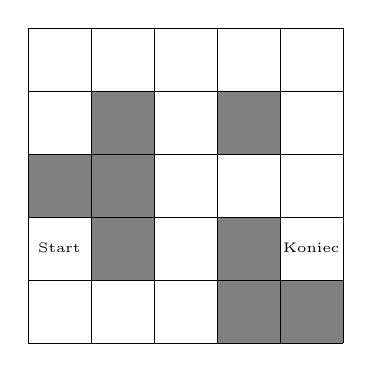
\begin{tikzpicture}[scale=0.8]
        \fill[gray] (1,2) rectangle ++(1,1);
        \fill[gray] (1,3) rectangle ++(1,1);
        \fill[gray] (3,1) rectangle ++(1,1);
        \fill[gray] (3,3) rectangle ++(1,1);
        \fill[gray] (1,1) rectangle ++(1,1);
        \fill[gray] (0,2) rectangle ++(1,1);
        \fill[gray] (3,0) rectangle ++(1,1);
        \fill[gray] (4,0) rectangle ++(1,1);
        
        \node at (0.5,1.5) {\tiny Start};
        \node at (4.5,1.5) {\tiny Koniec};

        \draw[step=1cm,ultra thin,black] (0,0) grid (5,5);
    \end{tikzpicture}
    \caption{\centering Przykładowy labirynt 5x5 z zaznaczonym startem i końcem, gdzie białe pole - przejście, czarne - ściana.}
    \label{fig:example_maze}
\end{figure}

Można zauważyć, że taka struktura jest reprezentacją grafu, gdzie pola odpowiadają wierzchołkom, a krawędzie łączą sąsiadujące pola przejściowe. Reprezentacja labiryntu w~formie grafu została przedstawiona na rysunku \ref{fig:maze_graph}.

\begin{figure}[h]
    \centering
    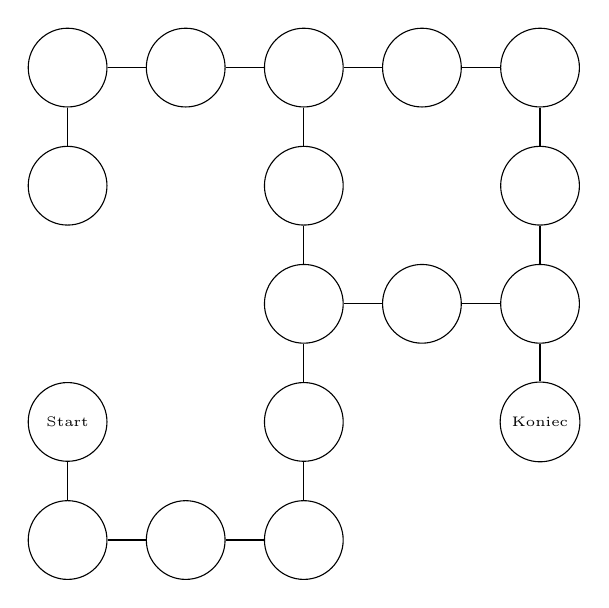
\begin{tikzpicture}[scale=1, every node/.style={circle,draw,minimum size=10mm}]
        \node (n00) at (0,0) {};
        \node (n01) at (0,1.5) {\tiny Start};
        \node (n03) at (0,4.5) {};
        \node (n04) at (0,6) {};

        \node (n10) at (1.5,0) {};
        \node (n14) at (1.5,6) {};

        \node (n20) at (3,0) {};
        \node (n21) at (3,1.5) {};
        \node (n22) at (3,3) {};
        \node (n23) at (3,4.5) {};
        \node (n24) at (3,6) {};

        \node (n32) at (4.5,3) {};
        \node (n34) at (4.5,6) {};

        \node (n41) at (6,1.5) {\tiny Koniec};
        \node (n42) at (6,3) {};
        \node (n43) at (6,4.5) {};
        \node (n44) at (6,6) {};

        \draw (n00) -- (n01);
        \draw (n03) -- (n04);
        \draw (n04) -- (n14);
        \draw (n00) -- (n10);
        \draw (n10) -- (n20);
        \draw (n20) -- (n21);
        \draw (n21) -- (n22);
        \draw (n22) -- (n23);
        \draw (n23) -- (n24);
        \draw (n14) -- (n24);
        \draw (n24) -- (n34);
        \draw (n41) -- (n42);
        \draw (n42) -- (n43);
        \draw (n43) -- (n44);
        \draw (n22) -- (n32);
        \draw (n32) -- (n42);
        \draw (n34) -- (n44);
    \end{tikzpicture}
    \caption{Graf reprezentujący labirynt z Rysunku \ref{fig:example_maze}.}
    \label{fig:maze_graph}
\end{figure}

W projekcie istotne jest porównanie różnych algorytmów wyszukiwania ścieżki, które pozwalają znaleźć trasę między dwoma punktami. W najlepszym przypadku celem jest znalezienie ścieżki \textit{optymalnej}, czyli takiej, która minimalizuje liczbę kroków, co w kontekście grafu o jednakowych wagach krawędzi sprowadza się do znalezienia drogi o minimalnej długości. Ścieżkę \textit{optymalną} oraz \textit{nieoptymalną} ukazuje rysunek \ref{fig:optimal_and_suboptimal_path}. 

\newpage

\begin{figure}[ht]
    \centering
    \begin{subfigure}{0.4\textwidth}
        \centering
        \begin{tikzpicture}[scale=0.8]
            \fill[gray] (1,2) rectangle ++(1,1);
            \fill[gray] (1,3) rectangle ++(1,1);
            \fill[gray] (3,1) rectangle ++(1,1);
            \fill[gray] (3,3) rectangle ++(1,1);
            \fill[gray] (1,1) rectangle ++(1,1);
            \fill[gray] (0,2) rectangle ++(1,1);
            \fill[gray] (3,0) rectangle ++(1,1);
            \fill[gray] (4,0) rectangle ++(1,1);

            \fill[pattern=north east lines, pattern color=green] (0,0) rectangle ++(1,1);
            \fill[pattern=north east lines, pattern color=green] (0,1) rectangle ++(1,1);
            \fill[pattern=north east lines, pattern color=green] (1,0) rectangle ++(1,1);
            \fill[pattern=north east lines, pattern color=green] (2,0) rectangle ++(1,1);
            \fill[pattern=north east lines, pattern color=green] (2,1) rectangle ++(1,1);
            \fill[pattern=north east lines, pattern color=green] (2,2) rectangle ++(1,1);
            \fill[pattern=north east lines, pattern color=green] (2,3) rectangle ++(1,1);
            \fill[pattern=north east lines, pattern color=green] (2,4) rectangle ++(1,1);
            \fill[pattern=north east lines, pattern color=green] (3,4) rectangle ++(1,1);
            \fill[pattern=north east lines, pattern color=green] (4,4) rectangle ++(1,1);
            \fill[pattern=north east lines, pattern color=green] (4,3) rectangle ++(1,1);
            \fill[pattern=north east lines, pattern color=green] (4,2) rectangle ++(1,1);
            \fill[pattern=north east lines, pattern color=green] (4,1) rectangle ++(1,1);

            \node at (0.5,1.5) {\tiny Start};
            \node at (4.5,1.5) {\tiny Koniec};

            \draw[step=1cm,ultra thin,black] (0,0) grid (5,5);
        \end{tikzpicture}
        \caption{Ścieżka nieoptymalna}
    \end{subfigure}
    \begin{subfigure}{0.4\textwidth}
        \centering
        \begin{tikzpicture}[scale=0.8]
            \fill[gray] (1,2) rectangle ++(1,1);
            \fill[gray] (1,3) rectangle ++(1,1);
            \fill[gray] (3,1) rectangle ++(1,1);
            \fill[gray] (3,3) rectangle ++(1,1);
            \fill[gray] (1,1) rectangle ++(1,1);
            \fill[gray] (0,2) rectangle ++(1,1);
            \fill[gray] (3,0) rectangle ++(1,1);
            \fill[gray] (4,0) rectangle ++(1,1);

            \fill[pattern=north east lines, pattern color=green] (0,0) rectangle ++(1,1);
            \fill[pattern=north east lines, pattern color=green] (0,1) rectangle ++(1,1);
            \fill[pattern=north east lines, pattern color=green] (1,0) rectangle ++(1,1);
            \fill[pattern=north east lines, pattern color=green] (2,0) rectangle ++(1,1);
            \fill[pattern=north east lines, pattern color=green] (2,1) rectangle ++(1,1);
            \fill[pattern=north east lines, pattern color=green] (2,2) rectangle ++(1,1);
            \fill[pattern=north east lines, pattern color=green] (3,2) rectangle ++(1,1);
            \fill[pattern=north east lines, pattern color=green] (4,2) rectangle ++(1,1);
            \fill[pattern=north east lines, pattern color=green] (4,1) rectangle ++(1,1);

            \node at (0.5,1.5) {\tiny Start};
            \node at (4.5,1.5) {\tiny Koniec};

            \draw[step=1cm,ultra thin,black] (0,0) grid (5,5);
        \end{tikzpicture}
        \caption{Ścieżka optymalna}
    \end{subfigure}
    \caption{Porównanie ścieżek w labiryncie.}
    \label{fig:optimal_and_suboptimal_path}
\end{figure}